%%%%%%%%%%%%%%%%%%%%% Chapter 14 %%%%%%%%%%%%%%%%%%%%%%%%%%%%%%%%%
% Privacy Post-Quantum: Securing the Future
%%%%%%%%%%%%%%%%%%%%%%%%%%%%%%%%%%%%%%%%%%%%%%%%%%%%%%%%%%%%%%%%%
\motto{To be future-proof, a trustworthy system must resist not only the adversaries of today but the quantum computers of tomorrow.}

\chapter{Privacy Post-Quantum: Securing the Future}
\label{chap:post_quantum}

\abstract{The advent of practical quantum computing poses an existential threat to the cryptographic foundations of modern AI. Protocols that currently protect Federated Learning, Secure Aggregation, and TEEs are largely based on mathematical problems that a quantum computer could solve in minutes. This chapter explores the "Post-Quantum" landscape for the Trustworthy AI Architect. We analyze Lattice-Based Cryptography and other quantum-resistant primitives, and discuss how to transition our existing secure distributed systems toward a "Quantum-Safe" future without sacrificing the efficiency and utility of our AI models.}

\section{The Quantum Threat}
\label{sec:quantum_threat}

Current asymmetric encryption (like RSA and ECC) and key exchange protocols (like Diffie-Hellman) depend on the difficulty of factoring large numbers or computing discrete logarithms. \textbf{Shor's Algorithm} has already proven that a sufficiently large quantum computer can solve these problems in polynomial time. For the Trustworthy AI Architect, this means that every encrypted update sent in a Federated Learning loop today could be recorded by a "Harvest Now, Decrypt Later" attacker and eventually exposed.

\section{Lattice-Based Cryptography for AI}
\label{sec:lattice_crypto}

The primary defense against the quantum threat is \textbf{Post-Quantum Cryptography (PQC)}. The most promising candidate for AI systems is \textbf{Lattice-Based Cryptography}. Unlike integer factorization, the problem of finding the shortest vector in a high-dimensional lattice remains computationally difficult for both classical and quantum computers.

Lattice-based schemes are particularly well-suited for AI because they can be used to construct \textbf{Fully Homomorphic Encryption (FHE)}, allowing for complex mathematical operations on encrypted model weights.

\begin{figure}[h]
\centering
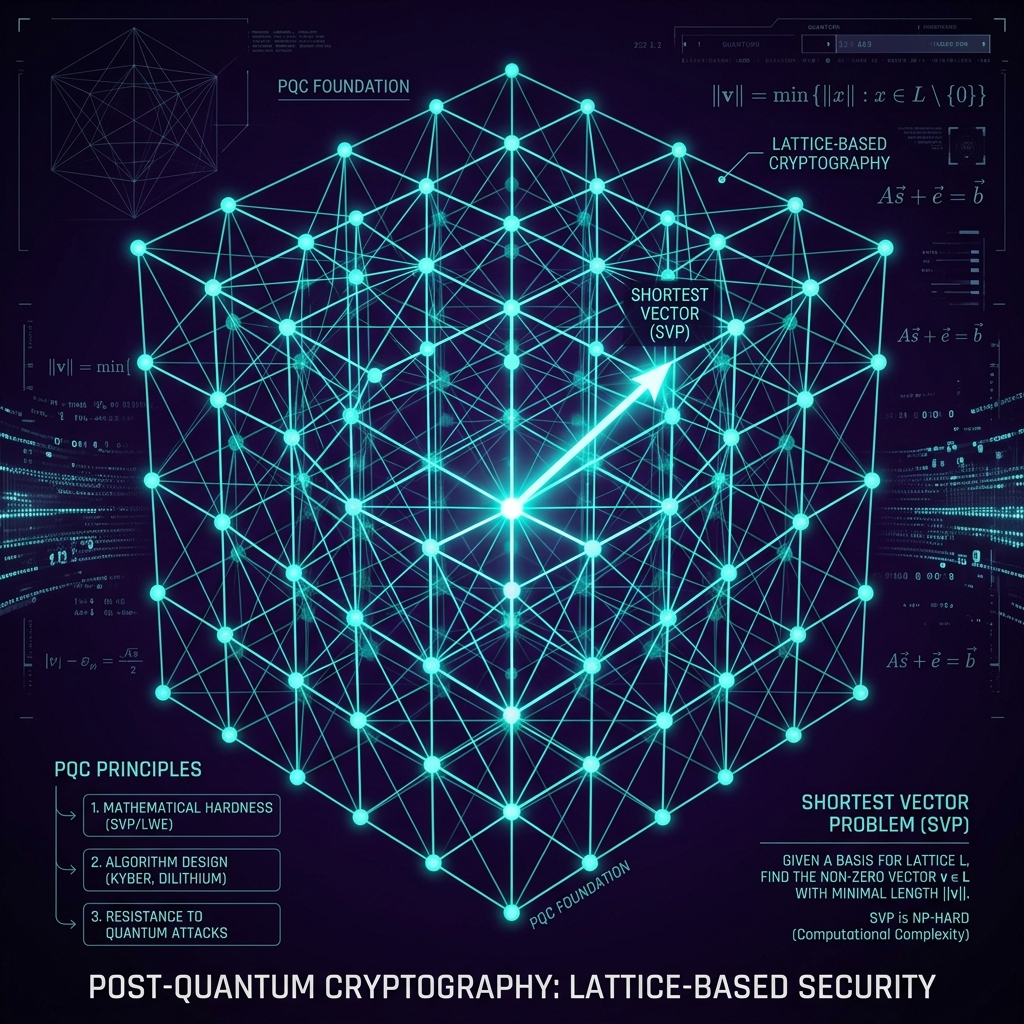
\includegraphics[width=0.8\textwidth]{figures/ch13_lattice.png}
\caption{Post-Quantum Foundations: A visualization of a mathematical lattice and the Shortest Vector Problem (SVP), which forms the basis for quantum-resistant AI security.}
\label{fig:ch13_lattice}
\end{figure}

\section{The Path to Quantum-Safe AI}
\label{sec:quantum_safe_transition}

Transitioning to a quantum-safe architecture requires two major shifts:

\begin{enumerate}
    \item \textbf{Hybrid Cryptography:} During the transition period, architects should use a "hybrid" approach that combines a classical protocol (for immediate security) with a post-quantum protocol (for future-proofing).
    \item \textbf{Hardware Agility:} TEEs and secure enclaves (as discussed in Chapter 9) must be updated to support PQC primitives at the instruction set level to minimize the performance overhead of lattice-based operations.
\end{enumerate}

\section{Conclusion}
\label{sec:conclusion_quantum}

Post-quantum privacy is the final defense in our "Model Robustness" toolkit. By securing the cryptographic foundations of our systems against future threats, we ensure that the trust we build today is enduring. In the next chapter, we look at how to maintain this trust in highly efficient, resource-constrained environments through the lens of \textbf{Efficient AI}.


